\documentclass[12pt, a4paper, titlepage, hidelinks]{scrreprt}	
%% UTF-8 File Encoding
\usepackage[utf8]{inputenc}
\usepackage[T1]{fontenc}

%% Language settings
\usepackage[ngerman]{babel}

\usepackage{fullpage}
\usepackage{graphicx}
\usepackage{caption}
\usepackage{subcaption}
\usepackage{placeins}
\usepackage{wrapfig}
\usepackage{url}
\usepackage[raiselinks=true, bookmarks=true, bookmarksopenlevel=1, bookmarksopen=true, bookmarksnumbered=true, hyperindex=true, plainpages=false, pdfpagelabels=true]{hyperref}
\usepackage{fancyhdr}
\usepackage[nottoc]{tocbibind}
\usepackage[usenames, dvipsnames]{color}
\usepackage{xcolor}
\usepackage{textcomp} 
\usepackage{fancybox}
\usepackage{mathtools}
\usepackage{csquotes}
\usepackage{dirtree}

\usepackage{tikz}
\usetikzlibrary{arrows, positioning, fit}

\graphicspath{{images/}}

\usepackage{setspace}
\setstretch{1.4}

\usepackage[a4paper]{geometry}
\geometry{left=3.25cm,right=2.5cm,top=3.5cm,bottom=3.5cm,head=14.5pt,headsep=4ex}

\usepackage[pdftex]{thumbpdf}
\pdfcompresslevel=9

\setcounter{secnumdepth}{3}
\setcounter{tocdepth}{3}

\parindent 0cm
\parskip1.5ex plus0.5ex minus0.5ex
\clubpenalty = 10000
\widowpenalty = 10000
\displaywidowpenalty = 10000

%% Caption configurations
\usepackage{caption}
\DeclareCaptionFont{white}{\color{white}}
\DeclareCaptionFormat{listing}{\colorbox{gray}{\parbox{\textwidth}{#1#2#3}}}
\captionsetup{font=small}
%\captionsetup[lstlisting]{format=listing,labelfont=white,textfont=white}
\definecolor{lightgray}{rgb}{.9,.9,.9}
\definecolor{darkgray}{rgb}{.4,.4,.4}
\definecolor{purple}{rgb}{0.65, 0.12, 0.82}

%% Contents in pdf bookmark list
%% uses etoolbox
\makeatletter
\pretocmd{\tableofcontents}{%
  \if@openright\cleardoublepage\else\clearpage\fi
  \pdfbookmark[0]{\contentsname}{toc}%
}{}{}%
\makeatother

\usepackage{lmodern}

\usepackage[activate={true,nocompatibility},final,tracking=true,kerning=true,spacing=true,factor=1100,stretch=10,shrink=10]{microtype}
\microtypecontext{spacing=nonfrench}

\pagestyle{fancy}
\renewcommand{\chaptermark}[1]{\markboth{\thechapter.\ #1}{}}
\fancyhf{}
\fancyhead[LE,RO]{{\headfont\thepage}}
\fancyhead[LO]{\headfont\nouppercase{\rightmark}}

%% better syntax highlighting
\usepackage[chapter, outputdir=out]{minted}
\usemintedstyle{colorful} %https://raw.github.com/n1k0/SublimeHighlight/master/themes.png
\newcommand{\mintedfileinput}[2]{
\microtypesetup{protrusion=false}
\inputminted[frame=lines,framesep=7pt,linenos=false,numbersep=6pt,baselinestretch=1,xleftmargin=10pt, tabsize=2]{#1}{"../#2"}
\microtypesetup{protrusion=true}
}

\newcommand{\mintedfile}[4]{
\begin{listing}[H]
  \mintedfileinput{#1}{#2}
  \vspace{-16pt}
  \caption{#3}
  \label{#4}
\end{listing}
\vspace{-17pt}
}

\newcommand{\clicommand}[1]{\begin{quote}{\ttfamily \raggedright \noindent #1}\end{quote}}

\hypersetup{
 pdfauthor={Mathias Garbe},
 pdftitle={Projektarbeit Asteroids Dokumentation},
 pdfsubject={},
 pdfkeywords={}
}

\title{Projektarbeit Asteroids}
\subtitle{Dokumentation und Ausblick
\begin{figure}[h!]
  \centering
  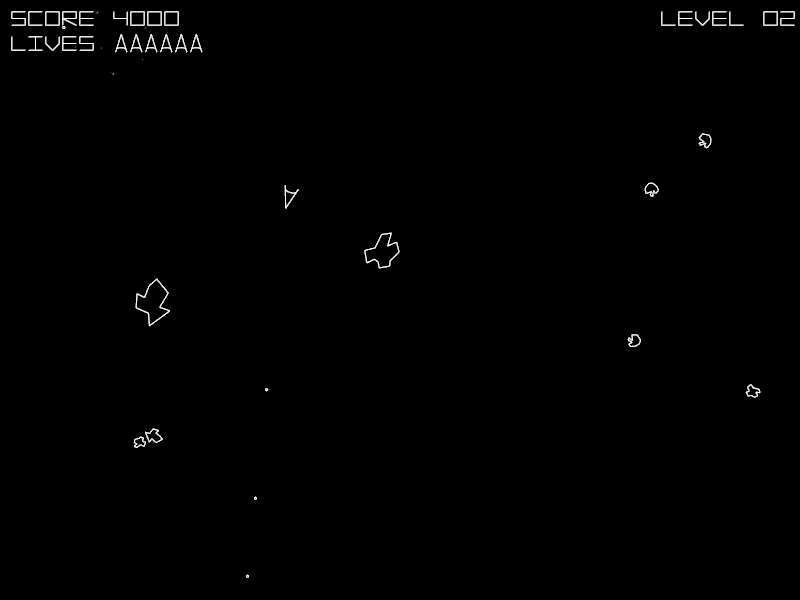
\includegraphics[width=\textwidth]{screenshot.png}
\end{figure}
}
\author{Mathias Garbe}

\begin{document}

\pagenumbering{roman}
\maketitle


\microtypesetup{protrusion=false}
\tableofcontents
\microtypesetup{protrusion=true}

\clearpage

\pagenumbering{arabic}

\chapter{Dokumentation}



\section{Überblick und Ordnerstruktur}

\dirtree{%
.1 /.
.2 cmake \DTcomment{Hilfsskripte für CMake}.
.3 VisualStudio \DTcomment{Visual Studio Solution Template}.
.2 data.
.3 shader \DTcomment{Shader-Quelldateien}.
.2 doc \DTcomment{Dokumentation}.
.3 de.
.2 src \DTcomment{Quelldateien}.
.3 Game \DTcomment{Logik des Spiels}.
.4 Components \DTcomment{Komponenten der Spiel-Entitäten}.
.3 Graphics \DTcomment{Grafik-Subsystem}.
.4 Geometry \DTcomment{Geometrie}.
.4 Shader \DTcomment{Shaderverwaltung}.
.4 Window \DTcomment{Fensterverwaltung}.
.3 Math \DTcomment{Mathe- und Vektorsubsystem}.
}

\section{Abhängigkeiten}

Das Projekt hat folgende Software-Abhängigkeiten:
\begin{itemize}
  \item CMake >=2.8 (Download von \url{http://www.cmake.org})
  \item GLFW >=3.0.4 (Download von \url{http://www.glfw.org})
  \item GLEW >=1.10.0 (Download von \url{http://glew.sourceforge.net})
\end{itemize}

Unter Linux sind diese Abhängigkeiten meist im jeweiligen Paket-Manager verfügbar und einfach zu installieren.

Auch ist ein C++11-fähiger Compiler notwendig. Dies ist unter Linux/Mac OS X \texttt{gcc} in Version 4.7 oder höher sowie \texttt{clang} in Version 3.0 oder höher und unter Microsoft Windows \texttt{Visual Studio 2013} oder höher. Zusätzlich wird noch eine Grafikkarte inklusiver passender Treiber benötigt die mit dem OpenGL 3 Core Profile kompatibel sind.

\section{Buildsystem}
Zum Bauen des Projekts wird CMake verwendet. CMake erzeugt aus den Skriptdateien (\texttt{CMakeFiles.txt}) Makefiles und Projektdateien für eine Reihe von IDEs. Im Zuge der Entwicklung wurden sowohl mit der Visual Studio Solution, Sublime Text Projekt und den GNU Makefiles gearbeitet.  

\subsection{Einrichten von CMake}
\label{cmake-setup}
Für den Fall dass die erforderten Abhängigkeiten nicht mit einem Paketmanager installiert wurden (oder unter Windows entwickelt wird) kann eine \texttt{UserDefinitions.cmake} im Hauptverzeichnis erstellt werden, mit welcher die Pfade von GLFW und GLEW angegeben werden können. Die Datei \texttt{UserDefinitions.cmake.example} kann dabei als Vorlange benutzt werden.

Der Inhalt der \texttt{UserDefinitions.cmake} in einer Windows-Entwicklungsumgebung könnte zum Beispiel so aussehen:

\mintedfile{cmake}{listings/UserDefinitions.cmake.windows}{Ein Beispiel für eine \texttt{UserDefinitions.cmake} unter Windows. Die Windows-Typischen umgekehrten Schrägstriche (Backslash) müssen dabei durch normale Schrägstriche ersetzt werden.}{lst:UserDefinitions.cmake}

Es ist darauf zu achten, dass die \texttt{UserDefinitions.cmake} nicht in die Versionsverwaltung eingecheckt wird, da sie für jede Entwicklungsumgebung spezifisch ist. Deswegen ist diese Datei auch in der \texttt{.gitignore} aufgeführt.

\subsection{Kompilieren des Projekts}
Um die Projektdateien zu bauen öffnet man am einfachsten die Konsole und wechselt in das Projektverzeichnis. Dort können dann mit den folgenden Befehlen die Projektdateien erzeugt werden:
\clicommand{>~mkdir~build\\ >~cd~build\\ >~cmake~..}

Anstatt \texttt{>~cmake ..} zu benutzen kann auch mit \texttt{>~cmake-gui} eine grafische Oberfläche ausgeführt werden, über welche nun CMake eingerichtet werden kann. Falls CMake die Abhänigkeiten GLFW oder GLEW nicht finden kann so wird dies als Fehler ausgegeben und die Ausführung abgebrochen. In diesem Fall muss eine \texttt{UserDefinitions.cmake} erstellt werden oder die Pfadangaben in einer vorhandenen überprüft werde (siehe \autoref{cmake-setup}).

\paragraph{Linux und Mac OS X}
Unter Linux und Mac OS X kann danach per \texttt{>~make} das Projekt gebaut werden. Das Spiel benötigt zum Ausführen Zugriff auf die Shader-Quelldateien, welche sich in \texttt{data/shader/} befinden. Da das Spiel diese Shader-Dateien relativ zum aktuellen Arbeitsverzeichnis erwartet, muss das Spiel im Hauptverzeichnis gestartet werden:
\clicommand{>~cd ~..\\ >~./build/src/asteroids}

Das Spiel wurde auch unter FreeBSD ohne Anpassungen des Quellcodes erfolgreich kompiliert und gespielt.

\paragraph{Windows}
Unter Windows kann die erstellte Visual Studio Solution mit Visual Studio 2013 geöffnet und das Projekt gebaut sowie gestartet werden. Die Einrichtung des korrekten Arbeitsverzeichnis hat CMake mithilfe einer Solution Template in \texttt{/cmake/VisualStudio/} übernommen und muss somit nicht von Hand erledigt werden.

\section{Klassenabhängigkeiten}
\begin{figure}[h!]
  \centering
  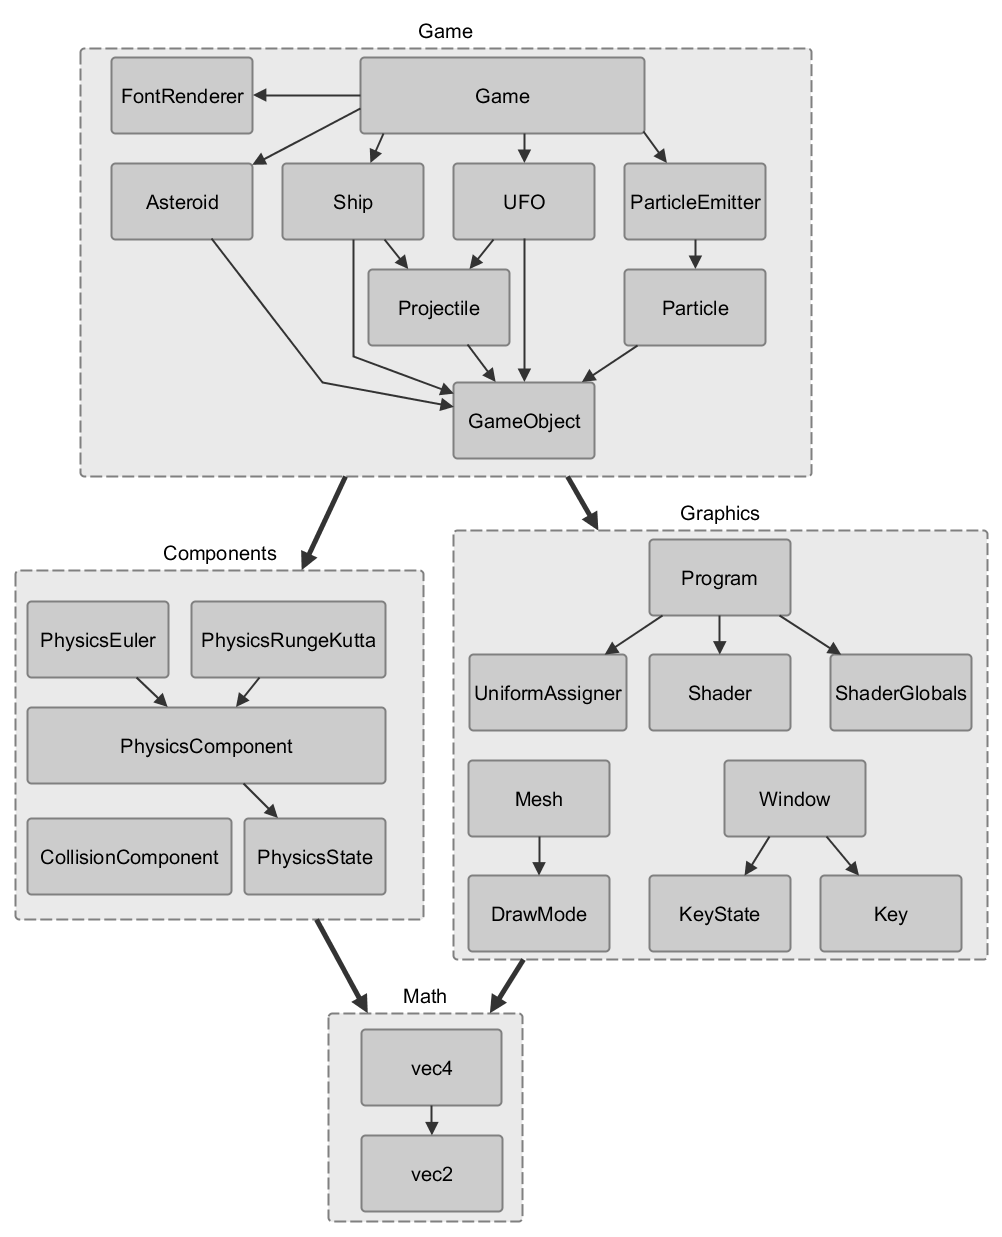
\includegraphics[width=\textwidth]{../graphs/dependency1.png}
\end{figure}

\section{Engine-Design}

Die Engine wurde komplett für das Asteroids-Spiel entworfen. Es wurden von Anfang an Entscheidungen getroffen, welche die Portabilität der Engine auf allen Plattformen sicherstellt. Auch wird das zugrundeliegende Grafiksystem abstrahiert um eine Portierung zu vereinfachen. In diesem Abschnitt sollen einige Kernaspekte vorgestellt und erläutert werden. 

\subsection{Hauptschleife}

Der große Unterschied von Videospielen zu ``normalen'' Programmen liegt nicht zuletzt in dem Vorhandensein einer Hauptschleife, welche erst mit Beenden des Spiels terminiert. Listing \autoref{lst:mainloop.cpp} zeigt die Hauptschleife des Asteroids-Spiels.

In dieser Hauptschleife wird zuerst das aktuelle Zeitdelta berechnet. Dieses Zeitdelta repräsentiert die Dauer der Verarbeitung des letzten Bildes. Um nun genau 60 Bilder pro Sekunde auszugeben müsste dieses Delta exakt 16,66 ms groß sein. Danach wird die Physik und Spiellogik aller Spielobjekte berechnet. Um den numerischen Fehler in der Physiksimulation sowie der Kollisionsabfrage und generell Darstellungsfehler zu vermeiden muss die Simulation mit festen Zeitschritten berechnet werden. Dazu wird das Zeitdelta zuerst auf eine Variable addiert, welche das gesamte Zeitbudget speichert. So werden auch Zeitdeltas berücksichtigt die kleiner als der feste Zeitschritt sind.

Anhand dieses gesamten Zeitbudgets werden dann so viele Simulationsschritte berechnet wie möglich sind. Dazu wird nach jedem Simulationsschritt der feste Zeitschritt von dem Zeitbudget abgezogen, und die Simulation so oft wiederholt solange das Zeitbudget größer als der feste Zeitschritt ist. Da auf langsameren Rechnern diese Simulation jedoch insgesamt zu viel Zeit in Anspruch nehmen kann und damit das Zeitdelta des nächsten Bildes vergrößert wird, was wiederum die Anzahl der Simulationsschritte erhöht, gibt es ein Limit von 30 Schritten pro ausgegebenen Bild. Dies führt zwar dazu, dass das Spiel insgesamt langsamer läuft, aber andererseits würde der Spieler ansonsten schon nach wenigen ausgegebenen Bildern ein Stillstand des Programms feststellen. Mehr Informationen sind auch im Blog von Glenn Fiedler\footnote{\url{http://gafferongames.com/game-physics/fix-your-timestep/}} zu finden.

Anschließend werden alle Spielobjekte und die Benutzeroberfläche gezeichnet. Zum Schluss wird das fertige Bild auf dem Bildschirm angezeigt.

\mintedfile{cpp}{listings/mainloop.cpp}{\texttt{src/Game/Game.cpp}: Die Hauptschleife des Spiels, welche sich unter anderem um die korrekte Simulation der Spiellogik kümmert indem diese mit festen Zeitschritten aufgerufen wird. So wird der Fehler der Physiksimulation minimiert und eine konstante Simulationsgeschwindigkeit erreicht.}{lst:mainloop.cpp}

\subsection{Fensterverwaltung}

Die Fensterverwaltung ist im Kern nur ein dünne API-Schicht für GLFWwindow, welches eine C-Bibliothek ist. Die \texttt{Window}-Klasse kümmert sich um das Erstellen eines Fensters beliebiger Größe und verwaltet den OpenGL-Kontext. Auch Tastatureingaben und die Mausposition werden hier verarbeitet und dem Spielcode zur Verfügung gestellt.

\mintedfile{cpp}{listings/Window.h}{\texttt{src/Graphics/Window/Window.h}: Abstraktion des \texttt{GLFWwindow} und die Bereitstellung von Tastatureingaben sowie Mausposition.}{lst:Window.h}

\subsection{Shaderverwaltung}

Da im OpenGL 3 Core Profile keine alten OpenGL-Befehle (\textit{Fixed-Function} Befehle) verfügbar sind und somit auch die Benutzung von Shadern vorgeschrieben ist, muss die Engine Shader unterstützen. Dazu sind die Shader simpel gehalten und Vertex- sowie Fragmentshader werden zusammen in einer Datei definiert und per \texttt{\#ifdef} entsprechend geschützt. Listing~\autoref{lst:shader.glsl} zeig so einen Beispielshader, bei dem Vertex- und Fragmentshader zusammen definiert werden. 

\mintedfile{glsl}{listings/shader.glsl}{In diesem Beispielshader sind Vertex- und Fragmentshader kombiniert in einer Datei.}{lst:shader.glsl}

Damit bestimmte Definitionen und Funktionen von allen Shadern benutzt werden können wird vor jedem Shader die Datei \texttt{data/shader/global.glsl} inkludiert. Dies geschieht automatisch. In dieser Datei wird zum Beispiel die Funktion \texttt{generateProjection} definiert, welche die aktuelle Projektionsmatrix berechnet. Auch wird dort das Speicherlayout fest definiert. So ist zum Beispiel die Position der Eckpunkte immer auf Speicherstelle \texttt{0}.

\subsection{Zeichnen von Geometrie}

Zum Zeichnen von Geometrie existiert eine \texttt{Mesh}-Klasse. Diese übernimmt nicht nur das Zeichnen einer festen 2D-Geometrie, sondern kann diese auch rotieren und skalieren. Auch die Hüllkörper (\textit{Bounding Box}) der Geometrie wird von dieser Klasse berechnet.

Intern wird dazu eine OpenGL Vertex Array Object benutzt (VAO), welcher aus einem Vertex Buffer Object (VBO) und einen Element Buffer Object (EBO) besteht. Das VAO fasst das VBO und EBO zusammen mit den eingestellten Attributen und Zustände in einem Objekt zusammen, so dass zum Zeichnen nur noch das VAO aktiviert werden muss. Das VBO speichert alle Eckpunkte (\textit{Vertices}) und das EBO speichert die Reihenfolge der Eckpunkte in der eigentlichen Geometrie.

Die Geometrie kann sowohl ganz gezeichnet werden, als auch nur Teile davon. Dies wird zum Beispiel bei der Flamme des Antriebs beim Spielerschiff benutzt, welche eigentlich Teil der Schiffsgeometrie ist aber nur beim Beschleunigen angezeigt wird.

\section{Spiel-Design}

Das Ziel des Spiels ist es, alle Asteroiden eines Levels komplett zu zerstören. Dazu kann das Spielerschiff Projektile verschießen, wobei die Anzahl der maximal aktiven Projektile begrenzt sind. Wenn das Level nach einer bestimmten Zeit nicht komplett von Asteroiden befreit wurde, erscheint ein UFO, welches auf den Spieler schießt. Pro abgeschossenen Asteroiden und UFO erhält der Spieler Punkte. Nach je 1000 Punkte erhält der Spieler ein neues Leben. Kollidiert der Spieler mit einem Asteroid oder einem (eigenen oder gegnerischen) Projektil verliert der Spieler ein Leben. Solange der Spieler noch Leben übrig hat erscheint der Spieler in der Mitte des Spielfeldes neu und ist für eine Zeit lang unverwundbar. Die Nummer der Asteroiden und somit auch die Schwierigkeitsstufe steigt mit jedem bestandenen Level.

\subsection{Objekte}

Alle Objekte im Spiel erben von der \texttt{GameObject}-Klasse (siehe Listing~\autoref{lst:GameObject.h}). Diese Klasse stellt die grundlegenden Funktionen jedes Spielobjektes bereit, wie etwa die \texttt{update}-Methode, welche die Logik des Objets implementiert. Auch wird das Objekt so per \texttt{draw}-Methode gezeichnet.

Jedes Objekt entscheidet selbst ob es eine Physik- und Kollisionskomponente besitzt. So sind auch die Methoden \texttt{collisionComponent} und \texttt{physicsComponent} zu implementieren. Dabei kann eine Referenz auf die jeweilige Komponente zurückgegeben werden oder aber ein \texttt{nullptr}, wenn diese Komponente nicht benutzt wird.

Die Kollision zweier Komponenten wird in der Basisklasse anhand der Kollisionskomponente berechnet. Sollte ein Objekt keine Kollisionskomponente besitzen so kann kein anderes Objekt mit ihm kollidieren.

\mintedfile{cpp}{listings/GameObject.h}{\texttt{src/Game/GameObject.h}: Basisklasse für alle Spieleobjekte, von der jedes Objekt ableiten muss. Es implementiert Kollisionsabfragen und gibt das Interface für das Zeichnen und Updaten vor.}{lst:GameObject.h}

\subsection{Komponenten}

Die Spiele-Objekte sind nach einem Komponenten-System entworfen worden. Das bedeutet, das die Objekte nicht von mehreren Klassen ableiten, welche zum Beispiel Physik und Kollisionen implementieren, sondern eine Referenz auf eine eigene Komponente beinhalten. Damit lassen sich Mehrfachvererbungsprobleme wie das Diamanten-Problem umgehen und gleichzeitig sehr unterschiedliche Objekte realisieren.

Im Moment gibt es nur zwei Komponenten-Typen, die Kollisions- und die Physik-Komponenten. Dieses System ist jedoch variabel und es lassen sich eine Vielzahl von weiteren Komponenten erdenken. So könnte zum Beispiel die Eingabe aus der \texttt{Game}-Klasse gelöst werden und in eine Eingabe-Komponente verschoben werden, welche dann vom Schiff benutzt wird. Auch sind verschieden starke KI-Komponenten für unterschiedliche UFO-Typen oder Schwierigkeitsgerade denkbar. Mit der Einführung einer KI-Komponente könnten selbst Asteroid eine KI erhalten, welche verschiedene Modis ausführen könnte. Zum Beispiel kann ein Asteroid sich um seine eigene Achse drehen, oder generell eine gekrümmte Flugbahn haben. Auch Gravitation könnte so abgebildet werden.

Weitere Anregungen und Erläuterungen sind auch auf GameProgrammingPatterns.com\footnote{\url{http://gameprogrammingpatterns.com/component.html}} und im Blog von Ray Wenderlich\footnote{\url{http://www.raywenderlich.com/24878/introduction-to-component-based-architecture-in-games}} zu finden.

\paragraph{Kollisions-Komponente}
Damit Spielobjekte miteinander Kollidieren können kann jedes Objekt eine Kollisions-Komponente beinhalten. Im Moment gibt es nur eine Komponente, welche zuerst mit einem AABB-Test (Axis-aligned Bounding Box) schnell entscheiden kann, ob eine aufwändigere Linie-zu-Linien Kollision berechnet werden muss. Ist dies der Fall, wird jede Linie jedes Objektes gegen jede Line des anderen Objets miteinander auf einen Schnittpunkt getestet. Mit diesem Verfahren kann eine pixelgenau Kollision, wie sie im Spiel erforderlich ist, erzielt werden.

\paragraph{Physik-Komponenten}
Für die Physik gibt es zwei unterschiedliche Komponenten. Für alle Objekte, die sich mit einer konstanten Geschwindigkeit bewegen reicht die Genauigkeit einer normalen Eulersche Integration aus. Da jedoch das spielergesteuerte Schiff keine konstante Geschwindigkeit hat und die Richtung sich oft ändert ist die numerische Genauigkeit der Euler-Komponente nicht mehr ausreichend. Dafür gibt es die etwas aufwändiger zu berechnende Runge-Kutta-Komponente, welche eine Runge-Kutta Integration der 4. Ordnung implementiert. Damit wird die Ungenauigkeit auf ein akzeptables Niveau gesenkt welche dem Spieler nicht mehr auffällt.

\chapter{Ausblick}

Diese Kapitel soll einen Ausblick auf Weiterentwicklungs-Potential in dem Engine- und Spieldesign geben.

\section{Portierung auf andere Grafiksysteme}

Das Grafiksystem ist unabhängig vom Spielecode. Alle OpenGL-Befehle werden von der Engine gekapselt, um das Portieren des Spiels auf andere Grafiksysteme wie SDL, Mantle oder DirectX zu vereinfachen. Da das Spiel auf OpenGL mithilfe von GLFW für die Fensterverwaltung und Tasteneingabe programmiert wurde befinden sich jedoch innerhalb der Engine Abhängigkeiten darauf. Jedoch wurden keine Konstanten aus OpenGL (wie \texttt{GL\_TRIANGLES} oder ähnliche) benutzt sondern in einem eigenem Enum verpackt.

\mintedfile{cpp}{listings/Mesh.h}{Alle OpenGL-Enums wurden in eigenen Enums verpackt, sodass der Spielecode keine Verweise auf OpenGL hat, hier zu sehen am Beispiel von \texttt{src/Graphics/Geometry/Mesh.h}.}{lst:Mesh.h}

Eine Variante um die Grafikengine auf ein anderes Grafiksystem zu portieren wird in diesem Kapitel vorgestellt. Mithilfe des Pimpl-Idioms (\textit{Pointer to Implementation}) kann das eigentliche Interface welches vom Spielecode benutzt wird unabhängig vom Grafiksystem verwendet werden und das Grafiksystem relativ einfach und schnell ausgetauscht werden, solange dies das Interface voll unterstützt. 

\paragraph{Portierung mithilfe des Pimpl-Idioms}
Anhand der Fensterverwaltung in der Engine kann die Idee des Pimpl-Idioms einfach verstanden werden. Angenommen in der Datei \texttt{Window.h} (siehe Listing~\autoref{lst:pimpl/Window.h}) wird das Interface zur Fensterverwaltung definiert und kann so von dem Spielecode benutzt werden.

\mintedfile{cpp}{listings/pimpl/Window.h}{\texttt{Window.h}: Definition des Interfaces ohne eigene Daten. Nur die Referenz auf die eigentliche Implementation ist vorhanden.}{lst:pimpl/Window.h}

Wie man eindeutig sieht hat die Klasse \texttt{Window} keinerlei privaten Daten, die man bei einer Fensterverwaltung erwarten würde. Lediglich ein privater \texttt{unique\_ptr} auf die vorwärts-deklarierte Klasse \texttt{WindowImpl} ist vorhanden. Wenn der Spielecode nun die Datei \texttt{Window.h} inkludiert gibt es keine Möglichkeit auf die internen Daten Einfluss zu nehmen, da die komplette Implementierung in einer noch nicht spezifizierten und auch privaten Klasse liegt.

Erst in der \texttt{Window.cpp} (siehe Listing~\autoref{lst:pimpl/Window.cpp}) wird dieser Typ \texttt{WindowImpl} spezifiziert. Je nachdem welches Grafiksytem im Buildsystem ausgewählt wurde werden hier unterschiedliche Implementation angezogen und inkludiert. Da die \texttt{WindowImpl}-Klasse nun spezifiziert ist kann sie auch von der Fensterverwaltung verwendet werden. Im Konstruktor wird eine neue \texttt{WindowImpl}-Instanz erzeugt und als Member initialisiert. Alle Argumente werden der Implementation weitergereicht. Ähnlich werden auch Funktionen wie \texttt{getCursorPosition} einfach auf der eigentlichen Implementation aufgerufen und ggf. der Rückgabewert weitergereicht.

\mintedfile{cpp}{listings/pimpl/Window.cpp}{\texttt{Window.cpp}: Das Interface wrappt sich um eine spezialisierte Implementationsklasse, welche im Konstruktor erstellt wird. Da die Implementation als \texttt{unique\_ptr} angelegt ist muss sich nicht um den Speicher gekümmert werden.}{lst:pimpl/Window.cpp}

Für jedes unterstützte Grafiksystem muss also eine eigene Implementierung programmiert werden, welche dann von dem \texttt{Window} benutzt wird. Dabei ist zu beachten, dass nur eine Implementierung gleichzeitig mit dem Projekt kompiliert werden kann, da alle den gleichen Klassennamen haben.

\mintedfile{cpp}{listings/pimpl/WindowImplGLFW.h}{\texttt{WindowImplGLFW.h}: Ein Beispiel für die Implementierungsdetails der Fensterverwaltung in GLFW. Da dies nicht Teil des öffentlichen Interfaces ist kann es nach belieben und ohne Rücksicht auf Rückwärtskompatibilität verändert werden. Hier als Header-Only-Implementierung zu Darstellungszwecken.}{lst:pimpl/WindowImplGLFW.h}

Weiter Informationen zu dem Pimpl-Idiom befinden sich unter anderem hier:
\begin{itemize}
\item \url{http://www.gotw.ca/gotw/028.htm}
\item \url{http://www.gotw.ca/gotw/024.htm}
\item \url{http://en.wikibooks.org/wiki/C%2B%2B_Programming/Idioms#Pointer_To_Implementation_.28pImpl.29}
\end{itemize}

Das Pimpl-Idiom löst somit einen großen Teil des Portierungsaufwandes, da neue Grafiksysteme hinzugefügt werden können ohne das Interface zu verändern. Somit kann der Spielecode unverändert bleiben. Leider ist das Anfangs erwähnte \texttt{DrawMode}-Enum, welches vom Spielecode benutzt wird, nun noch immer eine direkte Referenz auf die OpenGL-Konstanten. Dies lässt sich jedoch einfach lösen, indem man im öffentlichen Teil des Interfaces komplett auf die OpenGL-Konstanten verzichtet. Die eigentliche Implementation kann dann selber entscheiden, wie sie damit umgehen möchte. Sie könnte zum Beispiel diese Enums wieder in OpenGL-Konstanten umwandeln, oder mit einer \texttt{switch}-Anweisungen alle Fälle abdecken. 

Jedoch könnte auch argumentiert werden, dass man komplett auf das \texttt{DrawMode}-Enum verzichten sollte und dafür Funktionen wie \texttt{drawTriangles} und \texttt{drawLines} in das Interface einführen sollte. Das löst zwar einige Fälle und eliminiert somit einige Enums, jedoch gibt es zum Beispiel in der Fensterverwaltung (\texttt{src/Graphics/Window}) ein \texttt{Key}-Enum, der alle Tasten auf der Tastatur abbildet. Dieser könnte nur sehr schlecht als Funktionen abgebildet werden und muss dementsprechend erhalten bleiben.

\paragraph{CMake-Unterstützung für mehrere Grafiksysteme}
Da dieses Beispiel auf das Buildsystem angewiesen sind um die Definitionen wie zum Beispiel \texttt{USE\_GLFW} zu setzen, müssen auch die CMake-Skripts angepasst werden. Zum Beispiel könnte dafür eine Option \texttt{graphics-api} eingeführt werden. Siehe Listing~\autoref{lst:CmakeLists-option.txt}.

\mintedfile{cmake}{listings/CmakeLists-option.txt}{Ein Beispiel wie Optionen der \texttt{CMakeLists.txt} hinzugefügt werden können. Abhängig von den Optionen werden verschiedene Definitionen dem Compiler übergeben und verschiedene Dateien dem Projekt hinzugefügt.}{lst:CmakeLists-option.txt}

Diese Option kann wie folgt mit \texttt{cmake} benutzt werden, hier wird beispielsweise Mantle als Grafiksystem ausgewählt:
\clicommand{>~cmake~-DGRAPHICS-API=MANTLE~..}

\paragraph{Alternativen zum Pimpl-Idiom}
Eine Alternative zu dem Pimpl-Idiom sind \textit{Opaque-Pointer}, oder in Qt auch \textit{D-Pointer} genannt. Dieses Idiom versteckt interne Daten hinter einem anonymen \texttt{struct}, das nur aus der jeweiligen Implementatierung sichtbar ist. 

Genau wie beim Pimpl-Idiom gibt es im Interface wieder keine privaten Daten, außer einen \texttt{unique\_ptr} auf einen forwärts-deklarierten \texttt{struct}.  Siehe Listing~\autoref{lst:dpointer/Window.h}.

\mintedfile{cpp}{listings/dpointer/Window.h}{\texttt{Window.h}: Definition des Interfaces ohne eigene Daten. Nur die Referenz auf das private Datenstruct (der D-Pointer oder Opaque-Pointer)ist vorhanden.}{lst:dpointer/Window.h}

Pro Grafikssystem gibt es nun eine Implementierung für dieses Interface. Um trotzdem die erforderlichen, privaten Member zu haben stecken diese nun in einem \texttt{struct}, welches nur in der Implementierung definiert wird.

\mintedfile{cpp}{listings/dpointer/WindowGLFW.cpp}{\texttt{WindowGLFW.cpp}: Private Daten werden im \texttt{WindowDetail} gespeichert, welches nur in dieser Datei sichtbar und zugänglich ist. Ansonsten wird das komplette Interface in dieser Datei implementiert.}{lst:dpointer/WindowGLFW.cpp}

Das Buildsystem muss sich also darum kümmern die jeweils gewünschte Implementierung zu bauen. Genau wie beim Pimpl-Idiom auch ändert sich das Interface (und somit die Binärkompatibilität) nicht wenn sich die darunterliegende Implementierung geändert wird oder neue, private Member hinzukommen.

Weiter Informationen zu Opaque-Pointer befinden sich unter anderem hier:
\begin{itemize}
\item \url{http://qt-project.org/wiki/Dpointer}
\item \url{http://en.wikipedia.org/wiki/Opaque_pointer#C.2B.2B}
\end{itemize}

\section{Multithreading}

Multithreading hat mittlerweile in jedem großen Spiel Einzug gehalten um noch komplexere Welten und Grafiken in Echtzeit berechnen zu können. Auch in dem eher simplen Asteroids-Spiel gibt es Potential von mehreren Prozessorkernen zu profitieren.

Dieses Kapitel sollen einige Möglichkeiten für den Einsatz von Multithreading im Asteroids-Spiel erläutert werden. Dabei soll die Physik-Komponente und das Zeichnen der Spielwelt separiert werden.

In einer richtigen 3D-Engine wäre jedoch auch Multithreading in anderen Komponenten denkbar. So könnte zum Beispiel die Animation und inverse Kinematik von 3D-Objekten, aber auch die Entscheidung, welche Objekte sichtbar sind (Culling) auf mehrere Threads aufgeteilt werden.

\subsection{Pipelining}

\paragraph{Doppelpufferung (\textit{Double Buffering})}

Genau wie im Grafikbereich schon üblich kann eine Doppelpufferung die Performance im Spiel- und Physikcode drastisch erhöhen. Dabei wird das Konzept aus der Grafikwelt hier in die Physikkomponente übertragen. Jede Komponente hat zwei Puffer für ihre Position, wobei einer der beiden immer als Arbeitspuffer fungiert (\textit{Backbuffer}) und einer von der Grafikkomponente ausgelesen werden kann (\textit{Frontbuffer}). Um den neuen Zustand zu berechnen braucht die Physikkomponente jederzeit den vorherigen Zustand, welcher im Frontbuffer gespeichert wird. Da auch die Grafikkomponente genau wie die Physikkomponente nur aus diesem Puffer lesen und nicht in diesen Puffer schreiben entstehen an dieser Stelle keine Wettlaufsituationen. Der Backbuffer kann von der Physikkomponente ohne Synchronisation beschrieben werden, da die Grafikkomponente diesen Puffer nicht ausliest. Listing~\autoref{lst:Pipeline-Approach1.h} zeigt so einen Ansatz. Der aktuelle Zeiger auf den richtigen Frontbuffer wird dabei über ein \texttt{std::atomic<unsigned int>} gelöst, welchen den Index repräsentiert. Dabei muss aber mit entsprechenden Signalen drauf geachtet werden, dass der Physik-Thread nie mehr als einen Frame im voraus berechnet, da es sonst zu Wettlaufsituationen kommen kann.

\mintedfile{cpp}{listings/Pipeline-Approach1.h}{}{lst:Pipeline-Approach1.h}

\clearpage

\paragraph{Separater Grafikzustand}

Anstatt mit einem atomaren Index zwischen Front- und Backbuffer zu unterscheiden kann die Physikkomponente auch zu Beginn des Frames den alten Zustand kopieren und so der Grafikkomponente zur Verfügung stellen. In Listing~\autoref{lst:Pipeline-Approach2.h} ist dies anhand eines Beispiels zu sehen. Genau wie bei der Doppelpufferung muss auch hier drauf geachtet werden, dass die Physikkomponente nie mehr als einen Frame im voraus berechnet, da sonst der aktuell von der Grafikkomponente ausgelesen Zustand überschrieben wird. Es kann mit dieser Methode jedoch auf den atomaren Index verzichtet werden.

\mintedfile{cpp}{listings/Pipeline-Approach2.h}{}{lst:Pipeline-Approach2.h}

\clearpage

\subsection{Aufgabenplaner \textit{(Task Schedulers)}}

Eine weitere Möglichkeit wäre die eigentlich unabhängig voneinander stattfindenen Physikberechnungen der Spielobjekte in kleine Aufgaben (\textit{Tasks}) aufzuteilen und diese dann parallel abzuarbeiten. Dazu ist ein Aufgabenplaner (\text{Task Scheduler}) nötig, welcher alle Aufgaben zu Beginn eines Frames zusammenträgt und dann in mehreren Threads abarbeitet.

Listing~\autoref{lst:TaskScheduler.h} zeigt eine Beispielimplementation eines solchen Task Schedulers. In der \texttt{update}-Methode der Physikkomponenten wird zuerst überprüft, ob ein Neuberechnen der Position notwendig ist. Sollte dies der Fall sein so wird dem Phsyik-Scheduler eine Referenz auf die \texttt{updateWorker}-Methode (als \texttt{std::function}) per \texttt{schedule} überreicht. Dieser trägt auf diese Weise alle in diesem Frame zu erledigende Tasks von allen Physikkomponenten zusammen. Nun wird die \texttt{work()}-Methode aufgerufen und jeder einzelne Task wird asynchron per \texttt{std::async} aufgerufen. Da natürlich bei vielen Komponenten die Anzahl der Aufgaben leicht die Anzahl der Prozessorkerne überschreiten kann sollte hier drauf geachtet werden, dass immer nur eine begrenzte Anzahl an Tasks gleichzeitig laufen. Es ist davon auszugehen, das jeder Task einzeln betrachtet kaum Rechenleistung braucht und somit auch ein kleiner Overhead in der Verwaltung der Threads entstehen kann. Hier muss also mit der richtigen Anzahl an simultanen Threads experimentiert werden.

Alternativ zu \texttt{std::async} kann hier auch mit einem Threadpool gearbeitet werden. So werden beim Starten des Spiels eine von der Leistung des Rechners abhängige Anzahl an Threads gestartet und dem Threadpool hinzugefügt. Diese Threads schlafen nun, bis sie vom Task Scheduler eine Aufgabe übertragen bekommen. Sie werden dann aus dem Pool genommen und erst nach vollenden des Arbeitspakets wieder diesem hinzugefügt. Dies löst die Problematik der negativen Leistungsentwicklung bei zu vielen Threads.

\mintedfile{cpp}{listings/TaskScheduler.h}{Ein Beispiel für einen Task Scheduler, der alle Tasks der Physikkomponenten zusammenträgt und dann parallel abarbeitet.}{lst:TaskScheduler.h}

\subsection{Dedizierter Thread}
Wenn größere Mengen Daten zur Laufzeit nachgeladen werden müssen (\textit{Streaming}) bietet sich die Verwendung eines dedizierten Threads an. Bei einem Spiel mit einer offenen Spielwelt wird meist nicht die gesamte Spielwelt im Speicher gehalten sondern nur der aktuell vom Spieler unmittelbar erreichbare Teil. Falls der Spieler sich nun an den Rand dieses geladenen Teils bewegt wird der dedizierierte Thread aufgeweckt und lädt im Hintergrund einen neuen Teil der Spielwelt nach, sodass der Spieler ohne Ladezeiten oder Ruckler von einen Teil der Welt in den nächsten Teil der Welt bewegen kann. Der Thread wird danach wieder schlafen gelegt und wartet darauf, den nächsten Teil der Welt nachzuladen.

In dem Asteroid-Spiel ist diese Art von Multithreading jedoch nicht anwendbar, da keine großen Datenmengen zur Laufzeit nachgeladen werden müssen.
\end{document}